\documentclass[11 pt, twocolumn]{article}

\usepackage{hyperref}
\usepackage{titling}
\usepackage{amsmath,amssymb}
\usepackage{algorithm}
\usepackage[noend]{algpseudocode}
\usepackage[margin=0.8in]{geometry}
\usepackage{graphicx}
\usepackage{color}
\usepackage{enumitem}
\setlist[enumerate]{label*=\arabic*.}

\makeatletter
\def\BState{\State\hskip-\ALG@thistlm}
\makeatother

\setlength{\droptitle}{-5em}
\setlength{\columnsep}{2em}

\title{\textbf{GPU Monitoring tool for Reinforcement Learning algorithms}\\\Large CS236605 - Deep Learning, Computer Science Department\\Technion, Israel Institute of Technology}

\author{Ira Gorodovskaya, Alexey Tusov}
\date{Spring 2019}

\newcommand{\todo}[1]{{\color{red}}}
\newcommand{\algspace}{\hspace{\algorithmicindent}}

\begin{document}
\maketitle
\section{Abstract}
Graphics Processing Units (GPUs) can significantly accelerate the training process for many deep learning models. Training deep learning models involves compute-intensive matrix multiplication and other operations that can take advantage of a GPU's massively parallel architecture.

However in practice, average GPU utilization for deep learning jobs tends to be surprisingly low, mainly because of common made algorithms and without customization for used hardware accelerators.

In this paper, we present a practical method for monitoring GPU metrics for the Arcade Learning Environment (ALE) and use it to benchmark GPU utilization among different Reinforcement Learning algorithms and try to find dependence between learning performances and GPU utilization.


\section{Introduction}
We started our project by benchmarking Evolution Strategies (ES) algorithms beside reinforcement learning (RL) algorithms, trying to understand what can cause difference in performances, main and the significant difference we pointed was massive parallel execution in ES algorithms meanwhile RL algorithms can be parallel in some cases but in many scales less parallel then ES. This cause us to think about the accelerators utilization in learning algorithms.


Researches in reinforcement learning (RL) have relied heavily on empirical evaluation, making experiment turnaround time a key limiting factor. Despite this critical bottleneck, many reference implementations do not fulfill
the potential of modern computers for throughput.
Efforts to parallelize and accelerate deep RL algorithms have been underway for several years. Recently, (Horgan et al., 2018\cite{horgan2018distributed}) showed that a distributed, prioritized replay buffer can support faster
learning while using hundreds of CPU cores for simulation and a single GPU for training. The same work used increased batch sizes, with a brief study of the effect of
learning rate.


Based on GPU's architecture we assume that serial RL algorithms may not utilize all available computing power provided by the GPU. And we want to understand if better GPU utilization may cause better learning performances.
In this work, we provide our implementation for GPU runtime monitoring, this tool could help to improve leverage by maximize performance of multiple CPUs and single GPU system (we made also a compatibility to support multi GPU monitoring), in purpose to gain significant improvement in efficiency, scale of hardware utilization and hence in learning speed.


\section{Methods}
\subsection{GPU architecture}
Execution in GPUs made by calling kernel methods from user space in CPU's level, each user process can call multiple GPU's kernels in synchronic modes and asynhronic modes, multiplying user processes means multiplying GPU's concurrent executed kernels, each kernel executed in at least one Thread Block (TB) and all TBs executed in one Streaming Multiprocessor (SM), each 32 threads in one TB grouped in Wrap and executed in parallel command level context. GPU's architecture supports multiple number of SMs and they all shares same global GPU memory, user's code in CPU level copies memory from CPU's global memory to GPU's global memory.
Data copy could be done by DMA transfer, which requires pinned memory in CPU's global memory and CPU's low memory availability in large parallel executions could be a bottle neck for such mechanism. In addition, data may be transferred using unified memory, which requires additional page management and may cause and additional overhead.
\begin{figure}
\centering
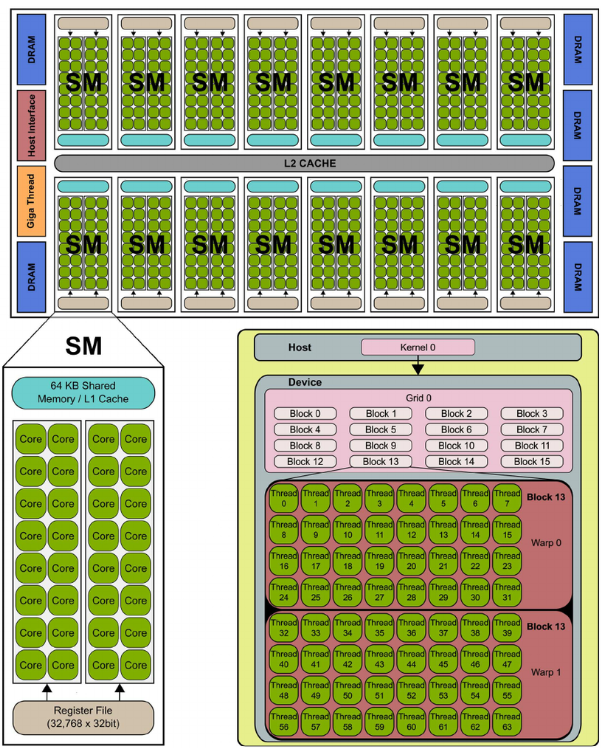
\includegraphics[width=0.93\columnwidth]{gpu_arch.png}
\caption{GPU architecture}
\vspace*{2pt}
\end{figure}

\subsection{RL algorithms}
In a standard reinforcement learning (RL) formulation as a Markov Decision Process, a learning agent aims to maximize the sum of discounted rewards experienced while interacting with an environment.
At each time step, the agent perceives the state of the environment and
takes an action, which causes the environment to transit into a new state. A scalar reward
signal evaluates the quality of each transition, and the agent has to maximize the cumulative reward along the course of interaction.

Next two sections provide a brief overview of several single-agent and multi-agent RL algorithms.

\subsection{Single Agent RL algorithms}
\textbf{DQN}: A reinforcement learning algorithm that was released by Google’s DeepMind, combines Q-Learning with deep neural networks to let RL work for complex, high-dimensional environments. \\
\textbf{Dueling DQN}: Splits the neural network into two — one learns to provide an estimate of the value at every timestep, and the other calculates potential advantages of each action, and the two are combined for a single action-advantage Q function.


\subsection{Multi-Agent RL algorithms}
In addition to benefits owing to the distributed nature of the multi-agent solution, such as the speedup made possible by parallel computation, multiple RL agents can harness new benefits from sharing experience, e.g., by communication, teaching, or imitation.

 \textbf{Asynchronous Advantage Actor-Critic (A3C)} consists of multiple independent agents (networks) with their own weights, who interact with a different copy of the environment in parallel. Thus, they can explore a bigger part of the state-action space in much less time.

Unlike DQN, where a single agent represented by a single neural network interacts with a single environment, A3C utilizes multiple incarnations of the above in order to learn more efficiently. In A3C there is a global network, and multiple worker agents which each have their own set of network parameters.
Each of these agents interacts with it’s own copy of the environment at the same time as the other agents are interacting with their environments. The reason this works better than having a single agent (beyond the speedup of getting more work done), is that the experience of each agent is independent of the experience of the others. In this way the overall experience available for training becomes more diverse.

The agents (or workers) are trained in parallel and update periodically a global network, which holds shared parameters. The updates are not happening simultaneously and that’s where the asynchronous comes from. After each update, the agents resets their parameters to those of the global network and continue their independent exploration and training for n steps until they update themselves again.


As an alternative to the asynchronous implementation, researchers found you can write a synchronous, deterministic implementation that waits for each agent to finish its segment of experience before performing an update, averaging over all of the agents. One advantage of this method is that it can more effectively use of GPUs, which perform best with large batch sizes. This algorithm is naturally called \textbf{A2C}, short for \textbf{Advantage Actor Critic}.


\begin{figure}
\centering
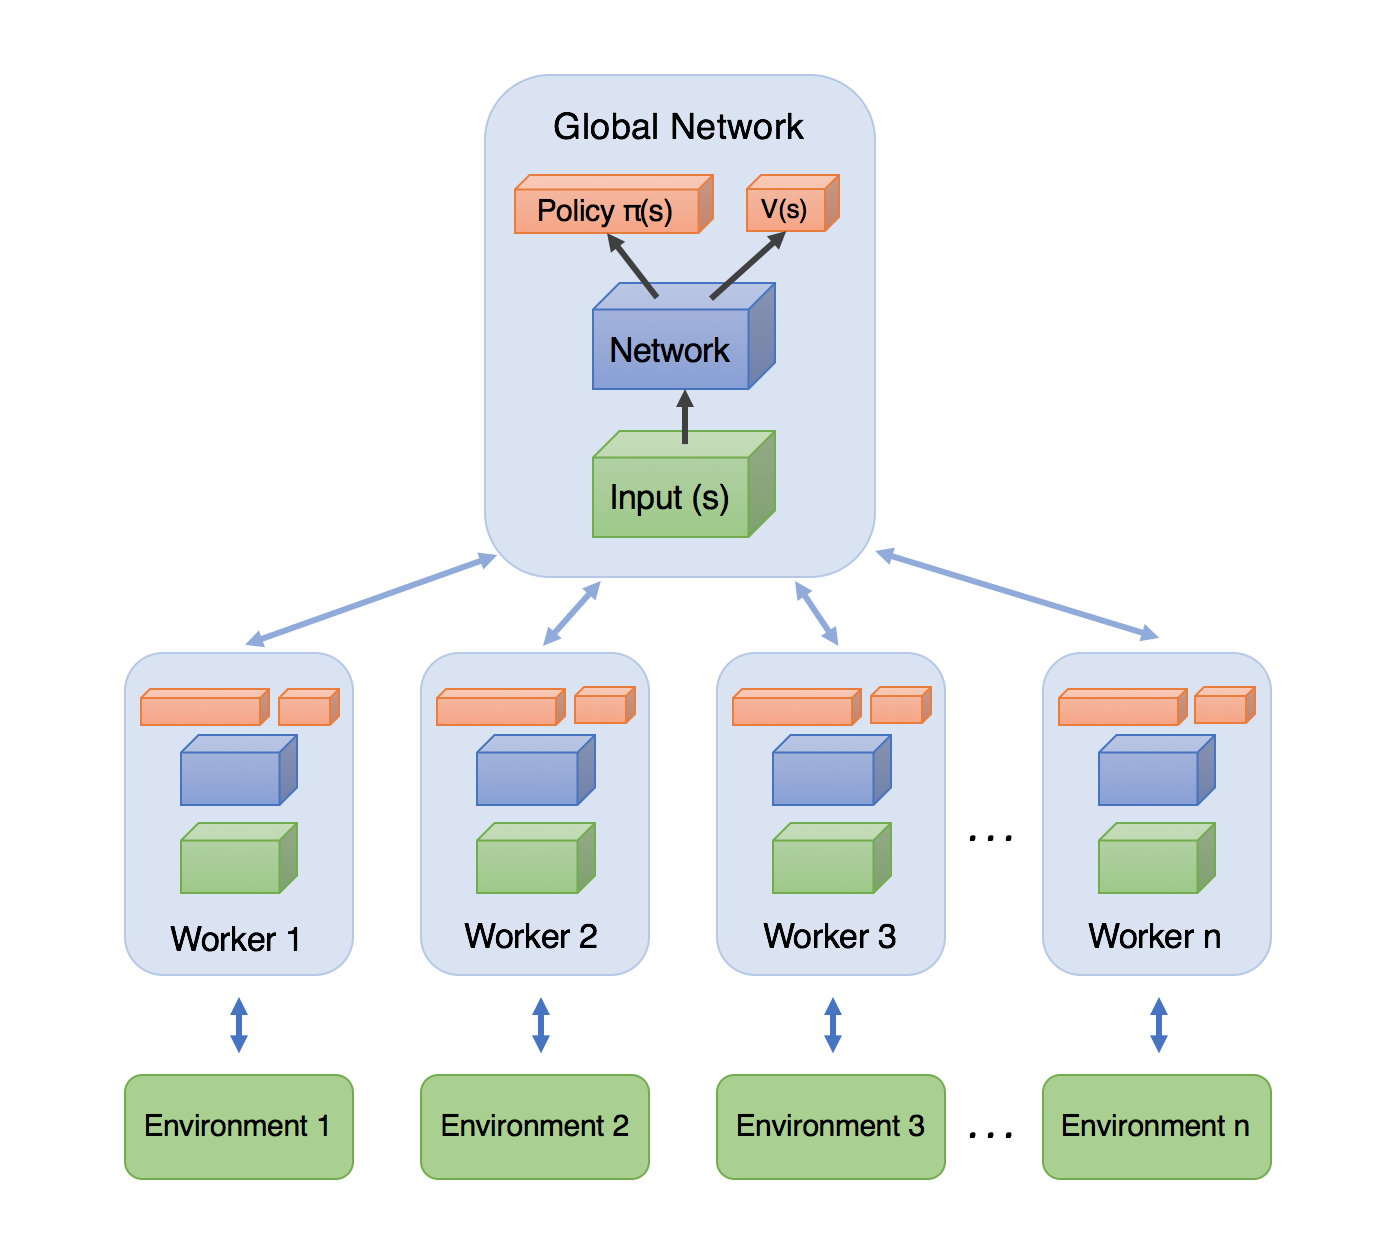
\includegraphics[width=0.93\columnwidth]{A3C.png}
\caption{Diagram of A3C high-level architecture}
\vspace*{2pt}
\end{figure}



\subsection{Data for evaluation}
For evaluation we prepared monitoring implementation of \textbf{A2C, DQN, DDQN, Dueling DQN and Rainbow} algorithms for Atari games learning, due to technical limitations we choose to use DQN and A2C algorithms to learn playing Atari game Pong.

\section{Implementation and Experiments}
Our implementation available online at \url{https://github.com/TusovAlexey/GPUMonitor}.


\subsection{GPUMonitor and GPUMonitorWrapper}

\textbf{GPUMonitor} is the main class for communication with GPUs and providing requested runtime information using \textbf{py3nvml} package, this class we used as reference from
torchlearning repository at  \url{https://github.com/chenyaofo/torchlearning}.
Supported GPU's real time information obtained:
\begin{enumerate}
\item Device name
\item Device memory
\begin{enumerate}
\item Total available memory [Mb]
\item Used memory [Mb]
\item Free memory [Mb]
\item List of used memory by different processes
\end{enumerate}
\item Temperature [Celsius]
\item Power
\begin{enumerate}
\item Used power [W]
\item Power limitation [W]
\end{enumerate}
\item Fan speed [Percent]
\item Utilization
\begin{enumerate}
\item GPU utilization [Percent]
\item GPU memory utilization [Percent]
\end{enumerate}
\end{enumerate}


\textbf{GPUMonitorWrapper} is a wrapper class for RL environments, this class inherits from Wrapper class and could be added to model's wrappers hierarchy. It's supports logging directly to ".csv" log file every episode using \textbf{ResultWriter} class. \textbf{GPUMonitorWrapper} is our implementation and R\textbf{esultWriter} class implemented by use with reference to Monitor class from bench package.

\subsection{RL agents}
We used as reference DeepRL-Tutorials repository at \url{https://github.com/goncamateus/DeepRL-Tutorials} for A2C, DQN, DDQN, Dueling DQN and Rainbow implementations for our agents implementation and experiments.

\subsection{Experiments}
We used DQN and A2C checking the following scenarios:
\begin{enumerate}
\item Comparing both models with default parameters
\item Checking influence CPUs number in A2C model
\item Checking influence of batch size in A2C model
\end{enumerate}
First of all we were interested to see if there is any confirmation for our assumption, better compute power utilization may lead to better learning performances, all our experiments done over PongNoFrameskip-v4 environment. Results are shown in Figure 2.
\begin{figure}
\centering
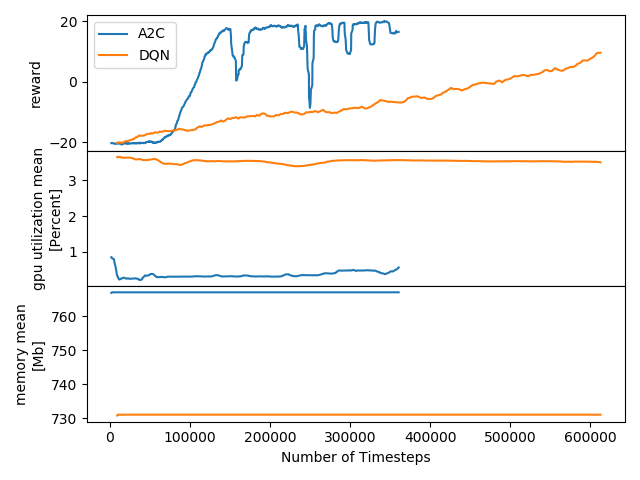
\includegraphics[width=0.93\columnwidth]{2c_32b.png}
\caption{Benchmarking different agents}
\vspace*{2pt}
\end{figure}



In our next experiment we focused on one model, we chose to focus on A2C model, before starting this experiment we assume that maybe the CPU is a bottle neck for increasing our compute power utilization, as we introduced in subsection 3.1 GPU architecture contains large amount of computing processors while the CPU have much less processors. Results are shown in Figure 3.
\begin{figure}
\centering
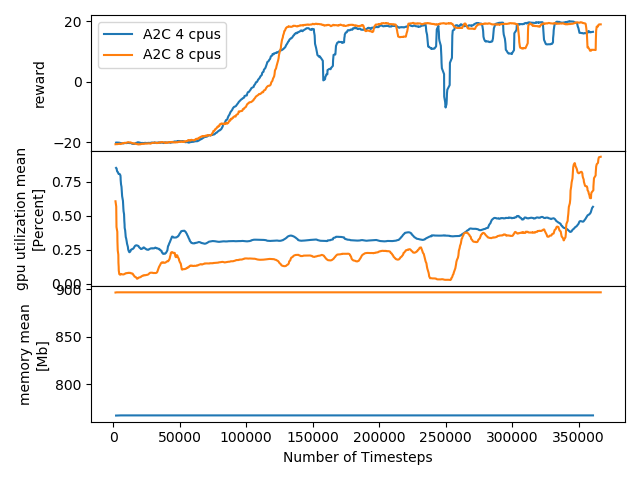
\includegraphics[width=0.93\columnwidth]{a2c_ncpus.png}
\caption{Benchmarking different number of CPUs}
\vspace*{2pt}
\end{figure}



In our last experiment we were interested if increasing the batch size may produce better performances. As we already seen, increasing utilization may increase learning performances, increasing batch size may also increase compute power utilization. For this experiment we used the same model of A2C agent and added additional execution with 512 batch size. Results are shown in figure 4.
\begin{figure}
\centering
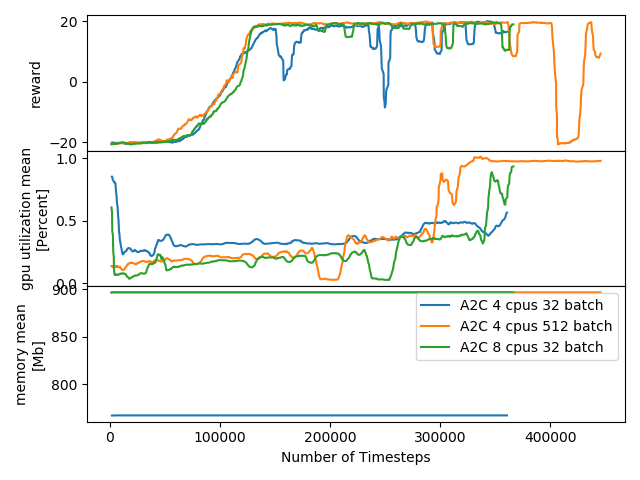
\includegraphics[width=0.93\columnwidth]{a2c_ncpus_nbatch.png}
\caption{Benchmarking different number of CPUs and increasing batch size}
\vspace*{2pt}
\end{figure}

\section{Results}
As seen in figure 2, our assumption may be partly confirmed, better GPU utilization would lead to faster learning. But regarding GPU utilization we expected to see different result, intuitively more utilized execution should use more compute power but based on constant value of used memory in DQN agent we can assume that high value of GPU utilization could be explained with high over head of memory transfers which are blocking other calculations or even maybe it's performs different matrix calculations.


Our second experiment results we can see almost similar learning performances, in one hand we can see that less CPUs may learn faster in specific period but on the other hand we can see that more CPUs reached highest score earlier, similar to our assumption, and stays more stable in well learned model. Surprisingly, the implementation with 8 CPUs utilize less GPU compute power then similar one with 4 CPUs, it may be due to the difference in memory usage, while the implementation with 4 CPUs may have an overhead of data migration due to lack of memory the 8 CPUs implementation shouldn't.


From our last experiment we conclude that increasing batch size may utilize more GPU compute power in some calculations but it shows almost same results as other implementations, this may be a good result for example where trying to increase compute power utilization may not always be worthwhile.


In conclusion, we established our assumption of increasing compute power utilization may lead to better learning performances meanwhile we seen that considerations regarding this increments should be considered well avoiding the reversed results.


In addition we hope this tool maybe useful for researchers benchmarking their models for overview where and how it can be better utilized.


%
%
%
%Our synchronous A2C implementation performs better than our asynchronous implementations — we have not seen any evidence that the noise introduced by asynchrony provides any performance benefit. This A2C implementation is more cost-effective than A3C when using single-GPU machines, and is faster than a CPU-only A3C implementation when using larger policies.
%
%
\bibliography{Refs}
\bibliographystyle{ieeetr}
\end{document}